\chapter{QMutableMapIterator}

template <typename Key, typename T> class QMutableMapIterator

QMutableMapIterator 类为 QMap 和 QMultiMap 提供 Java 风格的非常量迭代器。更多内容...

\begin{tabular}{|r|l|}
	\hline
	属性 & 方法 \\
	\hline
    头文件  &	\hl{\#include <QMutableMapIterator>} \\
    \hline
    qmake: & QT += core    \\
	\hline
\end{tabular}

\begin{compactitem}
\item 所有成员列表,包括继承的成员
\end{compactitem}

\section{公共成员函数}

\begin{longtable}{|r|m{28em}|}   
    \hline
    返回类型 	& 函数 \\
    \hline
    & QMutableMapIterator(QMap<Key, T> \emph{\&map}) \\
    \hline
    QMutableMapIterator<Key, T> \& &	operator=(QMap<Key, T> \emph{\&container}) \\
    \hline
    bool 	&findNext(const T \emph{\&value}) \\ 
    \hline
    bool 	&findPrevious(const T \emph{\&value}) \\
    \hline
    bool &	hasNext() const \\
    \hline
    bool 	&hasPrevious() const \\ 
    \hline
    const Key \& 	&key() const \\ 
    \hline
    QMutableMapIterator::Item &	next() \\ 
    \hline
    QMutableMapIterator::Item &	peekNext() const  \\
    \hline 
    QMutableMapIterator::Item &	peekPrevious() const \\ 
    \hline
    QMutableMapIterator::Item &	previous() \\ 
    \hline
    void &	remove() \\ 
    \hline
    void &	setValue(const T \emph{\&value}) \\ 
    \hline
    void &	toBack() \\ 
    \hline
    void &	toFront() \\ 
    \hline
    const T \& &	value() const \\
    \hline 
    T \&  &	value() \\ 
    \hline
\end{longtable}


\section{详细描述}

QMap 同时提供 Java 风格迭代器 和 STL 风格迭代器。
Java 风格迭代器比 STL 风格迭代器更高级,更容易使用;同时也略微低效。

QMutableMapIterator<Key, T> 用来遍历并修改 QMap (或 QMultiMap) 。
如果不想修改 map(或者 QMap 是 const 的),可以使用更快速的 QMapIterator。

QMutableMapIterator 构造函数接受 QMap 作为参数。
构造后,迭代器位于 map 的最开始位置(第一个元素之前)。
下面的例子演示如何顺序遍历所有元素:

\begin{lstlisting}[language=C++]
QMap<int, QWidget *> map;
...
QMutableMapIterator<int, QWidget *> i(map);
while (i.hasNext()) {
    i.next();
    qDebug() << i.key() << ": " << i.value();
}
\end{lstlisting}

next() 函数返回 map 中的下一个元素并将迭代器前移。
key() 和 value() 函数返回跳过的最后一个元素的键和值。

与 STL 风格迭代器不同,Java 风格迭代器指向元素之间而不是直接指向元素。
第一次调用 next() 前移迭代器到第一个和第二个元素之间的位置,并返回第一个元素;
第二次调用 next() 前移迭代器到第二个和第三个元素之间的位置;以此类推。

%%%%%%%%

\begin{figure}[hbt!]  
	\centering
    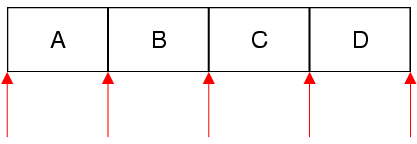
\includegraphics[width=0.5\textwidth]{javaiterators1}
	%\caption{model index}
\end{figure}


下面的例子演示如何反序遍历元素:

\begin{lstlisting}[language=C++]
QMutableMapIterator<int, QWidget *> i(map);
i.toBack();
while (i.hasPrevious()) {
    i.previous();
    qDebug() << i.key() << ": " << i.value();
}
\end{lstlisting}

如果想查找特定值的所有实例,循环使用 findNext() 或 findPrevious()。例如:

\begin{lstlisting}[language=C++]
QMutableMapIterator<int, QWidget *> i(map);
while (i.findNext(widget)) {
    qDebug() << "Found widget " << widget << " under key "
             << i.key();
}
\end{lstlisting}

如果想在遍历 map 时移除元素,使用 remove()。如果想修改元素的值,使用 setValue()。

例子:

\begin{lstlisting}[language=C++]
QMutableMapIterator<QString, QString> i(map);
while (i.hasNext()) {
    i.next();
    if (i.key() == i.value())
        i.remove();
}
\end{lstlisting}


该示例移除所有键和值相等的键值对。

任何时候,对于给定 map,只能有一个活动的可修改迭代器。
而且,当迭代器处于活动状态时,不可以直接修改 map,因为这会使迭代器失效,并导致未定义行为。

\begin{seeAlso}
QMapIterator 和 QMap::iterator。
\end{seeAlso}

\section{成员函数文档}

bool QMutableMapIterator::findPrevious(const T \emph{\&value})

从当前迭代器位置开始向后查找值 value。
如果找到值为 value 的键值对,返回 true;否则返回 false。

调用该函数后,如果找到值,迭代器将被移动到匹配元素的前面;
否则,迭代器将被移动到容器的前端。

\begin{seeAlso}
findNext()。
\end{seeAlso}

bool QMutableMapIterator::findNext(const T \emph{\&value})

从当前迭代器位置开始向前查找值 \emph{value}。
如果找到值为 \emph{value} 的键值对,返回 true;否则返回 false。

调用该函数后,如果找到值 \emph{value},迭代器将被移动到匹配元素的后面;否则,迭代器将被移动到容器的末端。

\begin{seeAlso}
findPrevious()。
\end{seeAlso}

const Key \&QMutableMapIterator::key() const

调用遍历函数(next(),previous(),findNext(),findPrevious())后,
该函数返回跳过的最后一个元素的键。

调用 next() 或 findNext() 后,key() 与 peekPrevious().key() 相同。
调用 previous() 或 findPrevious() 后,key() 与 peekNext().key() 相同。

\begin{seeAlso}
value()。
\end{seeAlso}

T \&QMutableMapIterator::value()

这是一个重载函数。

返回调用遍历函数后跳过的最后一个元素值的非常量引用。

QMutableMapIterator::Item QMutableMapIterator::peekPrevious() const

不移动迭代器而返回前一个元素。

对返回值调用 key() 获取元素的键,调用 value() 获取元素的值。

对位于容器前端的迭代器调用该函数将导致未定义结果。

\begin{seeAlso}
hasPrevious(),previous() 和 peekNext()。
\end{seeAlso}

QMutableMapIterator::Item QMutableMapIterator::previous()

返回前一个元素并将迭代器向后移动一个位置。

对返回值调用 key() 获取元素的键,调用 value() 获取元素的值。

对位于容器前端的迭代器调用该函数将导致未定义结果。

\begin{seeAlso}
hasPrevious(),peekPrevious() 和 next()。
\end{seeAlso}

bool QMutableMapIterator::hasPrevious() const

如果该迭代器前面至少有一个元素,返回 true,即该迭代器不在容器的前端;否则返回 false。

\begin{seeAlso}
hasNext() 和 previous()。
\end{seeAlso}

bool QMutableMapIterator::hasNext() const

如果该迭代器后面至少有一个元素,返回 true,即该迭代器不在容器的末端;否则返回 false。

\begin{seeAlso}
hasPrevious() 和 next()。
\end{seeAlso}

void QMutableMapIterator::toBack()

将迭代器移动到容器的末端(最后一个元素之后)。

\begin{seeAlso}
toFront() 和 previous()。
\end{seeAlso}

void QMutableMapIterator::toFront()

将迭代器移动到容器的前端(第一个元素之前)。

\begin{seeAlso}
toBack() 和 next()。
\end{seeAlso}

QMutableMapIterator<Key, T> \&QMutableMapIterator::operator=(QMap<Key, T> \&container)

将迭代器关联到 container 来遍历 map。
迭代器将被移动到 map 的前端(第一个元素之前)。

\begin{seeAlso}
toFront() 和 toBack()。
\end{seeAlso}

QMutableMapIterator::QMutableMapIterator(QMap<Key, T> \emph{\&map})

构造一个迭代器来遍历 \emph{map}。迭代器将被移动到 map 的前端(第一个元素之前)。

\begin{seeAlso}
operator=()。
\end{seeAlso}

QMutableMapIterator::Item QMutableMapIterator::next()

返回下一个元素并将迭代器向前移动一个位置。

对返回值调用 key() 获取元素的键,调用 value() 获取元素的值。

对位于容器末端的迭代器调用该函数将导致未定义结果。

\begin{seeAlso}
hasNext(),peekNext()和 previous()。
\end{seeAlso}

QMutableMapIterator::Item QMutableMapIterator::peekNext() const

不移动迭代器而返回下一个元素。

对返回值调用 key() 获取元素的键,调用 value() 获取元素的值。

对位于容器末端的迭代器调用该函数将导致未定义结果。

\begin{seeAlso}
hasNext(),next()和 peekPrevious()。
\end{seeAlso}

void QMutableMapIterator::remove()

移除使用遍历函数(next(),previous(),findNext(),findPrevious())跳过的最后一个元素。

\begin{seeAlso}
setValue()。
\end{seeAlso}

void QMutableMapIterator::setValue(const T \emph{\&value})

用 \emph{value} 替换使用遍历函数跳过的最后一个元素的值。

遍历函数包括 next(),previous(),findNext() 和 findPrevious()。

\begin{seeAlso}
key(),value() 和 remove()。
\end{seeAlso}

const T \&QMutableMapIterator::value() const

调用遍历函数(next(),previous(),findNext(),findPrevious())后,该函数返回跳过的最后一个元素的值。

调用 next() 或 findNext() 后,value() 与 peekPrevious().value() 相同。
调用 previous() 或 findPrevious() 后,value() 与 peekNext().value() 相同。

\begin{seeAlso}
key() 和 setValue()。
\end{seeAlso}